\documentclass[10pt, t]{beamer}
\usepackage{xcolor}
\usepackage{float}
\usepackage{extsizes}
% \usepackage{enumitem}
\usepackage{mathtools}
\usepackage{tikz}
\usepackage{subcaption}
% tables
\usepackage{multirow}
\usetikzlibrary{trees}

\mode<presentation>

%% ==== Theme and colors =====

%% manual colors
\definecolor{ctp_rosewater}{RGB}{245, 224, 220}
\definecolor{ctp_flamingo}{RGB}{242, 205, 205}
\definecolor{ctp_pink}{RGB}{245, 194, 231}
\definecolor{ctp_mauve}{RGB}{203, 166, 247}
\definecolor{ctp_red}{RGB}{243, 139, 168}
\definecolor{ctp_maroon}{RGB}{235, 160, 172}
\definecolor{ctp_peach}{RGB}{250, 179, 135}
\definecolor{ctp_yellow}{RGB}{249, 226, 175}
\definecolor{ctp_green}{RGB}{166, 227, 161}
\definecolor{ctp_teal}{RGB}{148, 226, 213}
\definecolor{ctp_sky}{RGB}{137, 220, 235}
\definecolor{ctp_sapphire}{RGB}{116, 199, 236}
\definecolor{ctp_blue}{RGB}{137, 180, 250}
\definecolor{ctp_lavender}{RGB}{180, 190, 254}
\definecolor{ctp_text}{RGB}{205, 214, 244}
\definecolor{ctp_subtext1}{RGB}{186, 194, 222}
\definecolor{ctp_subtext0}{RGB}{166, 173, 200}
\definecolor{ctp_overlay2}{RGB}{147, 153, 178}
\definecolor{ctp_overlay1}{RGB}{127, 132, 156}
\definecolor{ctp_overlay0}{RGB}{108, 112, 134}
\definecolor{ctp_surface2}{RGB}{88, 91, 112}
\definecolor{ctp_surface1}{RGB}{69, 71, 90}
\definecolor{ctp_surface0}{RGB}{49, 50, 68}
\definecolor{ctp_base}{RGB}{30, 30, 46}
\definecolor{ctp_mantle}{RGB}{24, 24, 37}
\definecolor{ctp_crust}{RGB}{17, 17, 27}

%% theme setup
\usetheme{CambridgeUS}
% \useinnertheme[shadow=True]{rounded}

\hypersetup{
    urlcolor=ctp_blue,
    colorlinks=true,
    linkcolor=.
}

%% colors

\setbeamercolor{background canvas}{bg=ctp_base} % backgroundgcc

\setbeamercolor{normal text}{fg=ctp_text}
\setbeamercolor{alerted text}{fg=ctp_red}
\setbeamercolor{example text}{fg=ctp_rosewater}
\setbeamercolor{math text}{fg=ctp_blue} %% changes the color of the math text

\setbeamercolor{palette primary}{bg=ctp_surface0, fg=ctp_red} % date
\setbeamercolor{palette secondary}{bg=ctp_base, fg=ctp_red} % title
\setbeamercolor{palette tertiary}{bg=ctp_red, fg=ctp_mantle}
\setbeamercolor{frametitle}{bg=ctp_text, fg=ctp_base}

% titlepage
\setbeamercolor{title}{bg=ctp_text, fg=ctp_base}
\setbeamercolor{author}{fg=ctp_text}
\setbeamercolor{institute}{fg=ctp_subtext1}
\setbeamercolor{date}{fg=ctp_subtext0}

% itemize items
\setbeamercolor{item}{fg=ctp_sapphire}
\setbeamercolor{subitem}{fg=ctp_sapphire}
\setbeamercolor{subsubitem}{fg=ctp_sapphire}

% figures and tables
\setbeamercolor{caption name}{fg=ctp_sapphire}
\setbeamercolor{section in toc}{fg=ctp_blue}
\setbeamercolor{subsection in toc}{fg=ctp_blue}

%% fonts
\setbeamerfont{date}{size=\scriptsize}
\setbeamerfont{subtitle}{size=\small}
\setbeamerfont{frametitle}{series=\bfseries}
% \setbeamerfont{date}{size=\footnotesize}

\setbeamerfont*{itemize/enumerate body}{size=\fontsize{9}{9}}
\setbeamerfont*{itemize/enumerate subbody}{size=\fontsize{8}{8}}
\setbeamerfont*{itemize/enumerate subsubbody}{size=\fontsize{7}{7}}

% \setbeamertemplate{blocks}[rounded][shadow=true]
% \setitemize{
%     label=\usebeamerfont*{itemize item}%
%     \usebeamercolor[fg]{itemize item}
%     \usebeamertemplate{itemize item}
% }

% \setbeamertemplate{itemize item}[square]
% \setbeamertemplate{itemize subitem}[ball]
% \setbeamertemplate{itemize subsubitem}[triangle]

\setbeamertemplate{itemize item}{\raisebox{0.22ex}{\rule{0.9ex}{0.9ex}}\hskip0.1em} % Square
\setbeamertemplate{itemize subitem}{\raisebox{0.12ex}{\textbullet}\hskip0.1em} % Ball
\setbeamertemplate{itemize subsubitem}{\raisebox{0.12ex}{\rule{0.4ex}{0.4ex}}\hskip0.1em} % Triangle
    
% hide footnote rule
\makeatletter
\def\beamer@autobreakframebox{%
    \global\setbox\beamer@splitbox=\box\voidb@x%
    \ifbeamer@autobreak%
        % Ok, frame was overful -> split it!
        \setbox\@tempboxa=\vsplit\beamer@framebox to\beamer@autobreakfactor\textheight%
        \global\setbox\beamer@splitbox=\box\beamer@framebox%
        \@tempdima=\ht\beamer@splitbox%
        \ifdim\@tempdima<\beamer@autobreaklastheight%
            \global\beamer@autobreaklastheight=\@tempdima\relax%
        \else%
            \setbox\@tempboxa=\vbox{\unvbox\@tempboxa\unvbox\beamer@splitbox}%
            \global\setbox\beamer@splitbox=\box\voidb@x%
        \fi%
        \setbox\beamer@framebox=\vbox to\textheight{\unvbox\@tempboxa%
            \vskip\beamer@framebottomskipautobreak%
            \ifvoid\beamer@splitbox%
                \ifvoid\beamer@footins%
                \else%
                    \begingroup
                        \usebeamercolor*[fg]{footnote}%
                        %\footnoterule%
                        \unvbox \beamer@footins%
                        \global\setbox\beamer@footins=\box\voidb@x%
                    \endgroup  
                \fi%
            \fi%
            \beamer@exitcode%
        }%
    \else%
        \setbox\beamer@framebox=\vbox to\textheight{\unvbox\beamer@framebox%
            \vskip\beamer@framebottomskip%
            \ifvoid\beamer@footins%
            \else%
                \begingroup
                    \usebeamercolor*[fg]{footnote}%
                    %\footnoterule%
                    \unvbox \beamer@footins%
                    \global\setbox\beamer@footins=\box\voidb@x%
                \endgroup 
            \fi%
            \beamer@exitcode
        }%
        \global\setbox\beamer@footins=\box\voidb@x%
    \fi%
}
\makeatother

% Adjust vertical alignment of itemize items
\makeatletter
\def\itemize{\@ifnextchar<{\beamer@inlineitemize}{\beamer@itemize}}
\makeatother

%% Macros
\newcommand{\indicatorname}[1]{\textcolor{ctp_green}{\textit{#1}}}
\newcommand{\changesize}[3]{\fontsize{#1}{#2}{#3}}

\title[Chatbot for any Website with RAG]{\textbf{{Custom Chatbot for any Website with Retrieval Augmented Generation}}}
\subtitle{Applied Machine Learning}
\author[R. Das, S. Sengupta, S, Saha, U. Dasgupta]{Roudranil Das \and Soham Sengupta \and Subhashree Saha \and Ujan Dasgupta}
\institute[CMI]{
    Chennai Mathematical Institute \\
    MSc. Data Science
}
\date{April 27, 2024}

\begin{document}

    \begin{frame}
        \titlepage
    \end{frame}

    \begin{frame}{Table of Contents}
        \tableofcontents
    \end{frame}

    \section{Introduction}
    \subsection{Problem statement}
    \begin{frame}{Problem statement}
        \begin{itemize}
            \item The objective is to create a natural language question answering chatbot on any given website (public or private)
            \item<2-> With the help of
            \begin{itemize}
                \item<2-> Large Language Models 
                \item<2-> LangChain
                \item<2-> Embeddings, Information retrieval and vector stores.
            \end{itemize}
        \end{itemize}
    \end{frame}

    \subsection{When to and not to apply LLM's}
    \begin{frame}{When to and not to apply LLM's}
        \begin{figure}
            \centering
            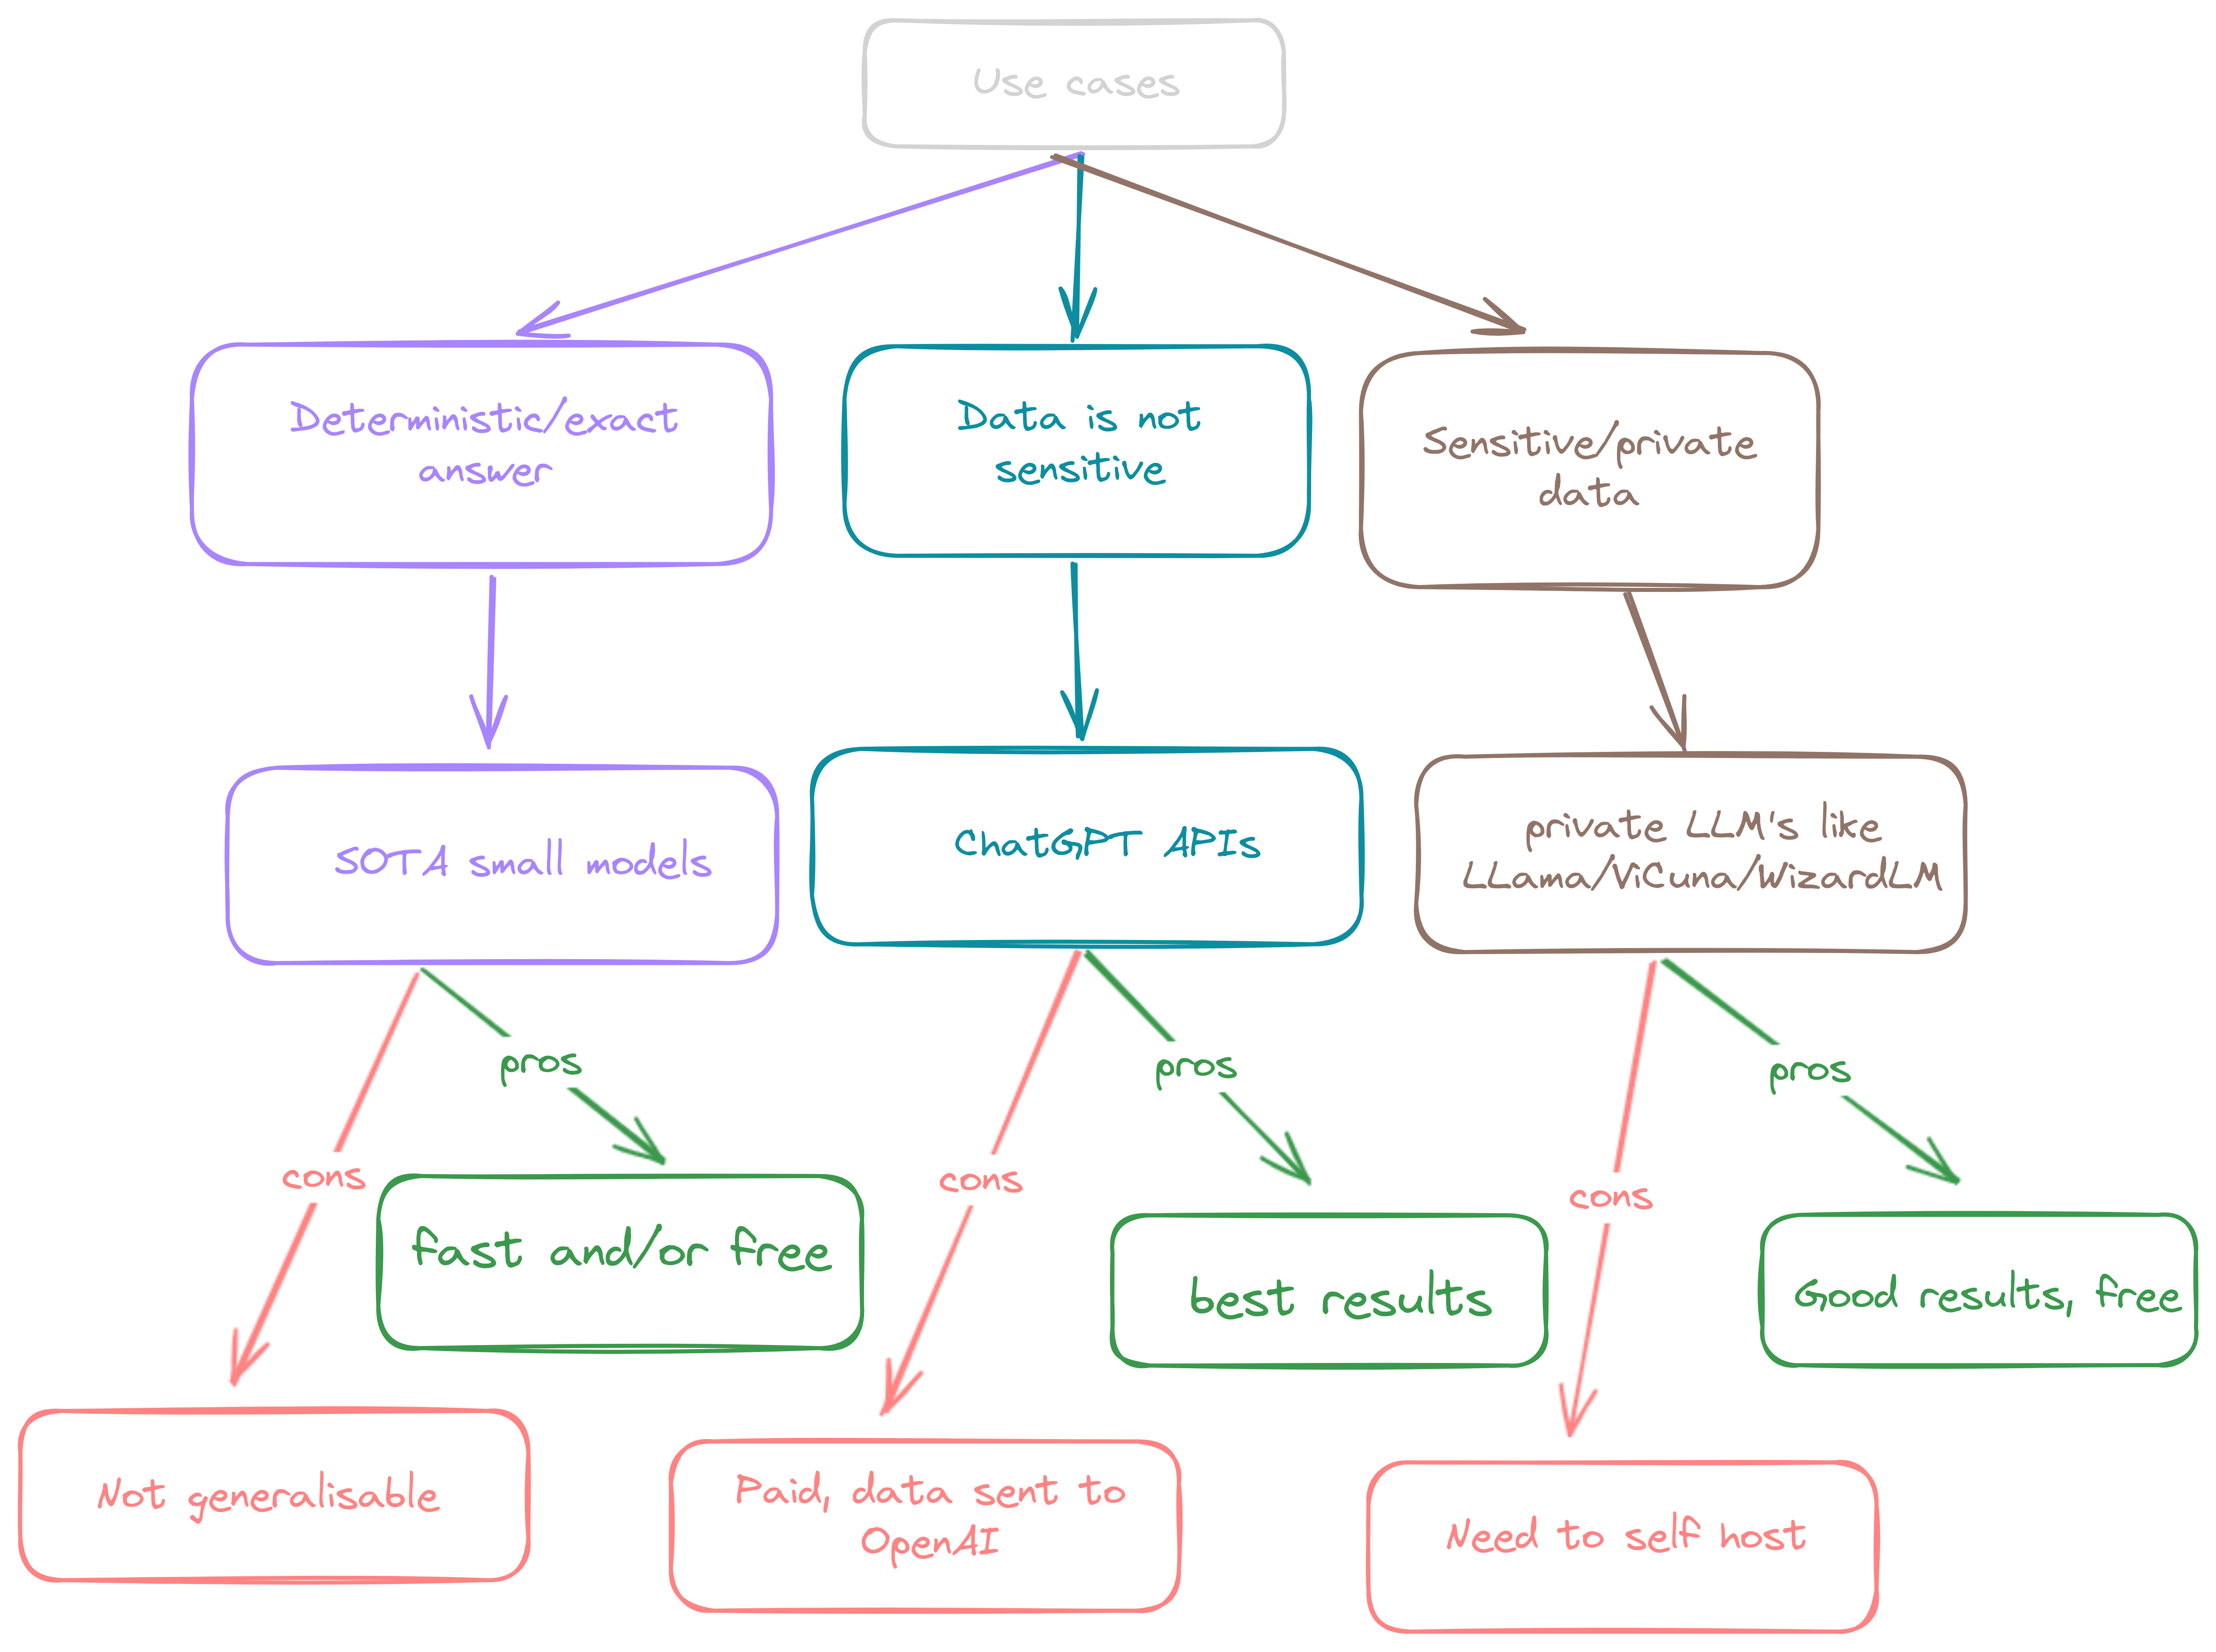
\includegraphics[height=0.8\textheight]{uc-1.png}
        \end{figure}
    \end{frame}

    \section{Creating the chatbot}
    \subsection{Data curation}
    \begin{frame}{Data curation}
        \begin{itemize}
            \item For our problem the data was curated from \href{https://en.wikibooks.org/wiki/Category:Recipes_with_metric_units}{Recipes around the world (wikibooks.com)}
            \begin{figure}[H]
                \centering
                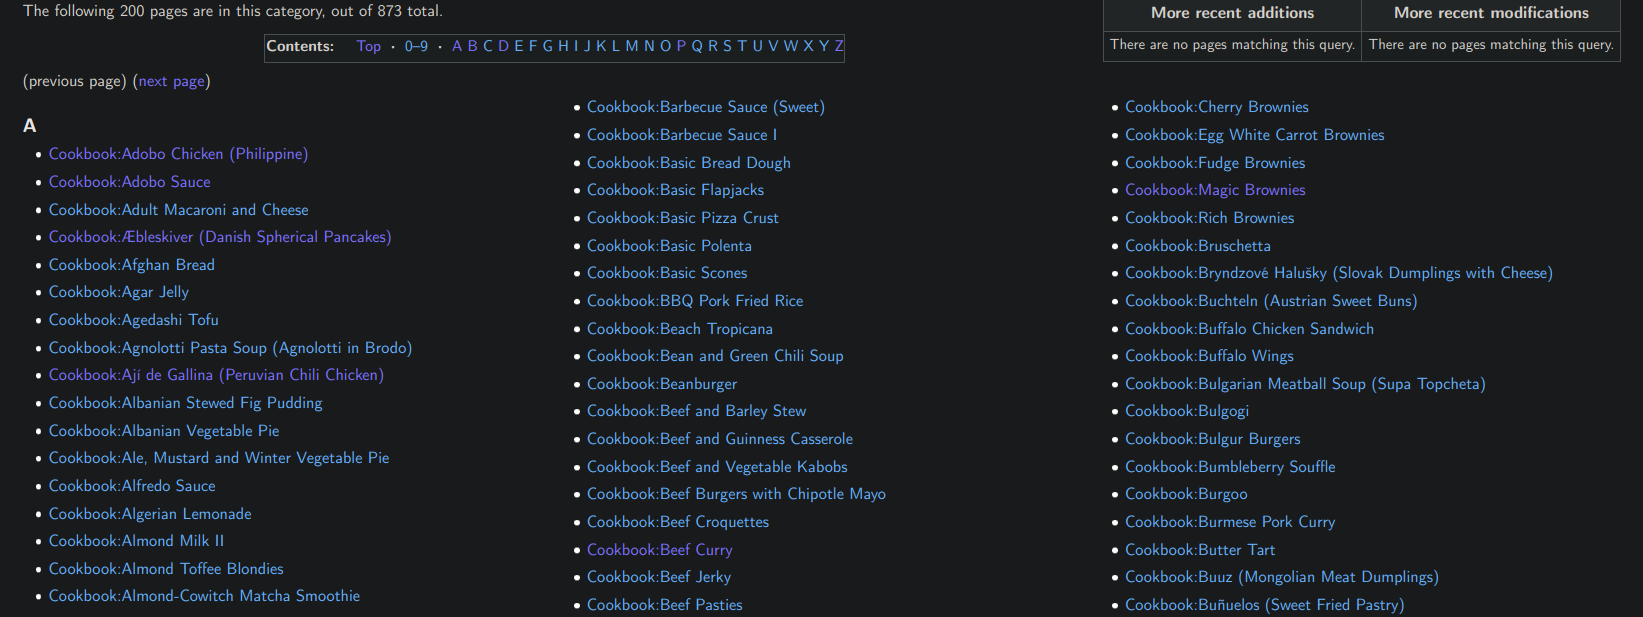
\includegraphics[width=0.8\textwidth]{recipes-website.png}
                \caption[]{Screenshot of how the recipes were in the website}
            \end{figure}
            \item Data collection: we used a web crawler (scrapy) to crawl all the pages on this site, extract the text and save them in a JSON file.
        \end{itemize}
    \end{frame}
    \begin{frame}{Data curation}
        \begin{figure}
            \centering
            \only<1>{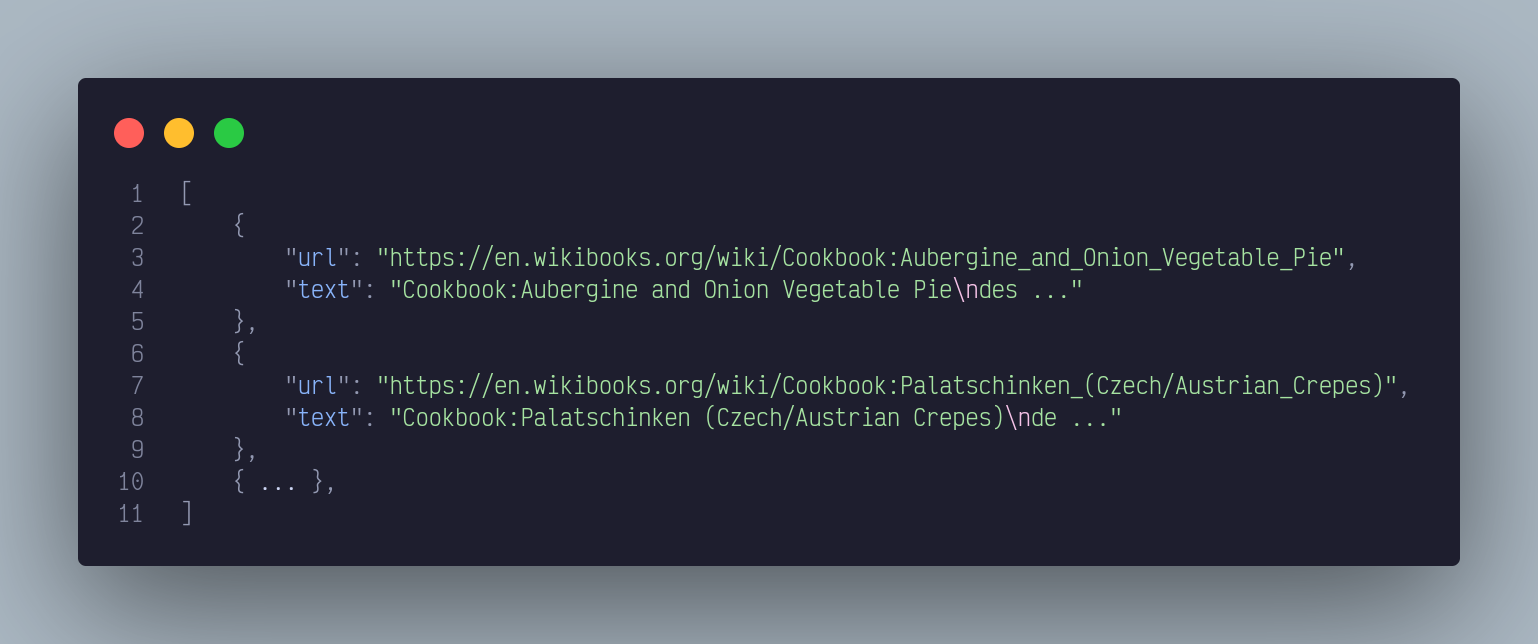
\includegraphics[width=0.8\textwidth]{samplejson.png}\caption[]{Preview of the JSON file where the recipes are saved.}}
            \only<2>{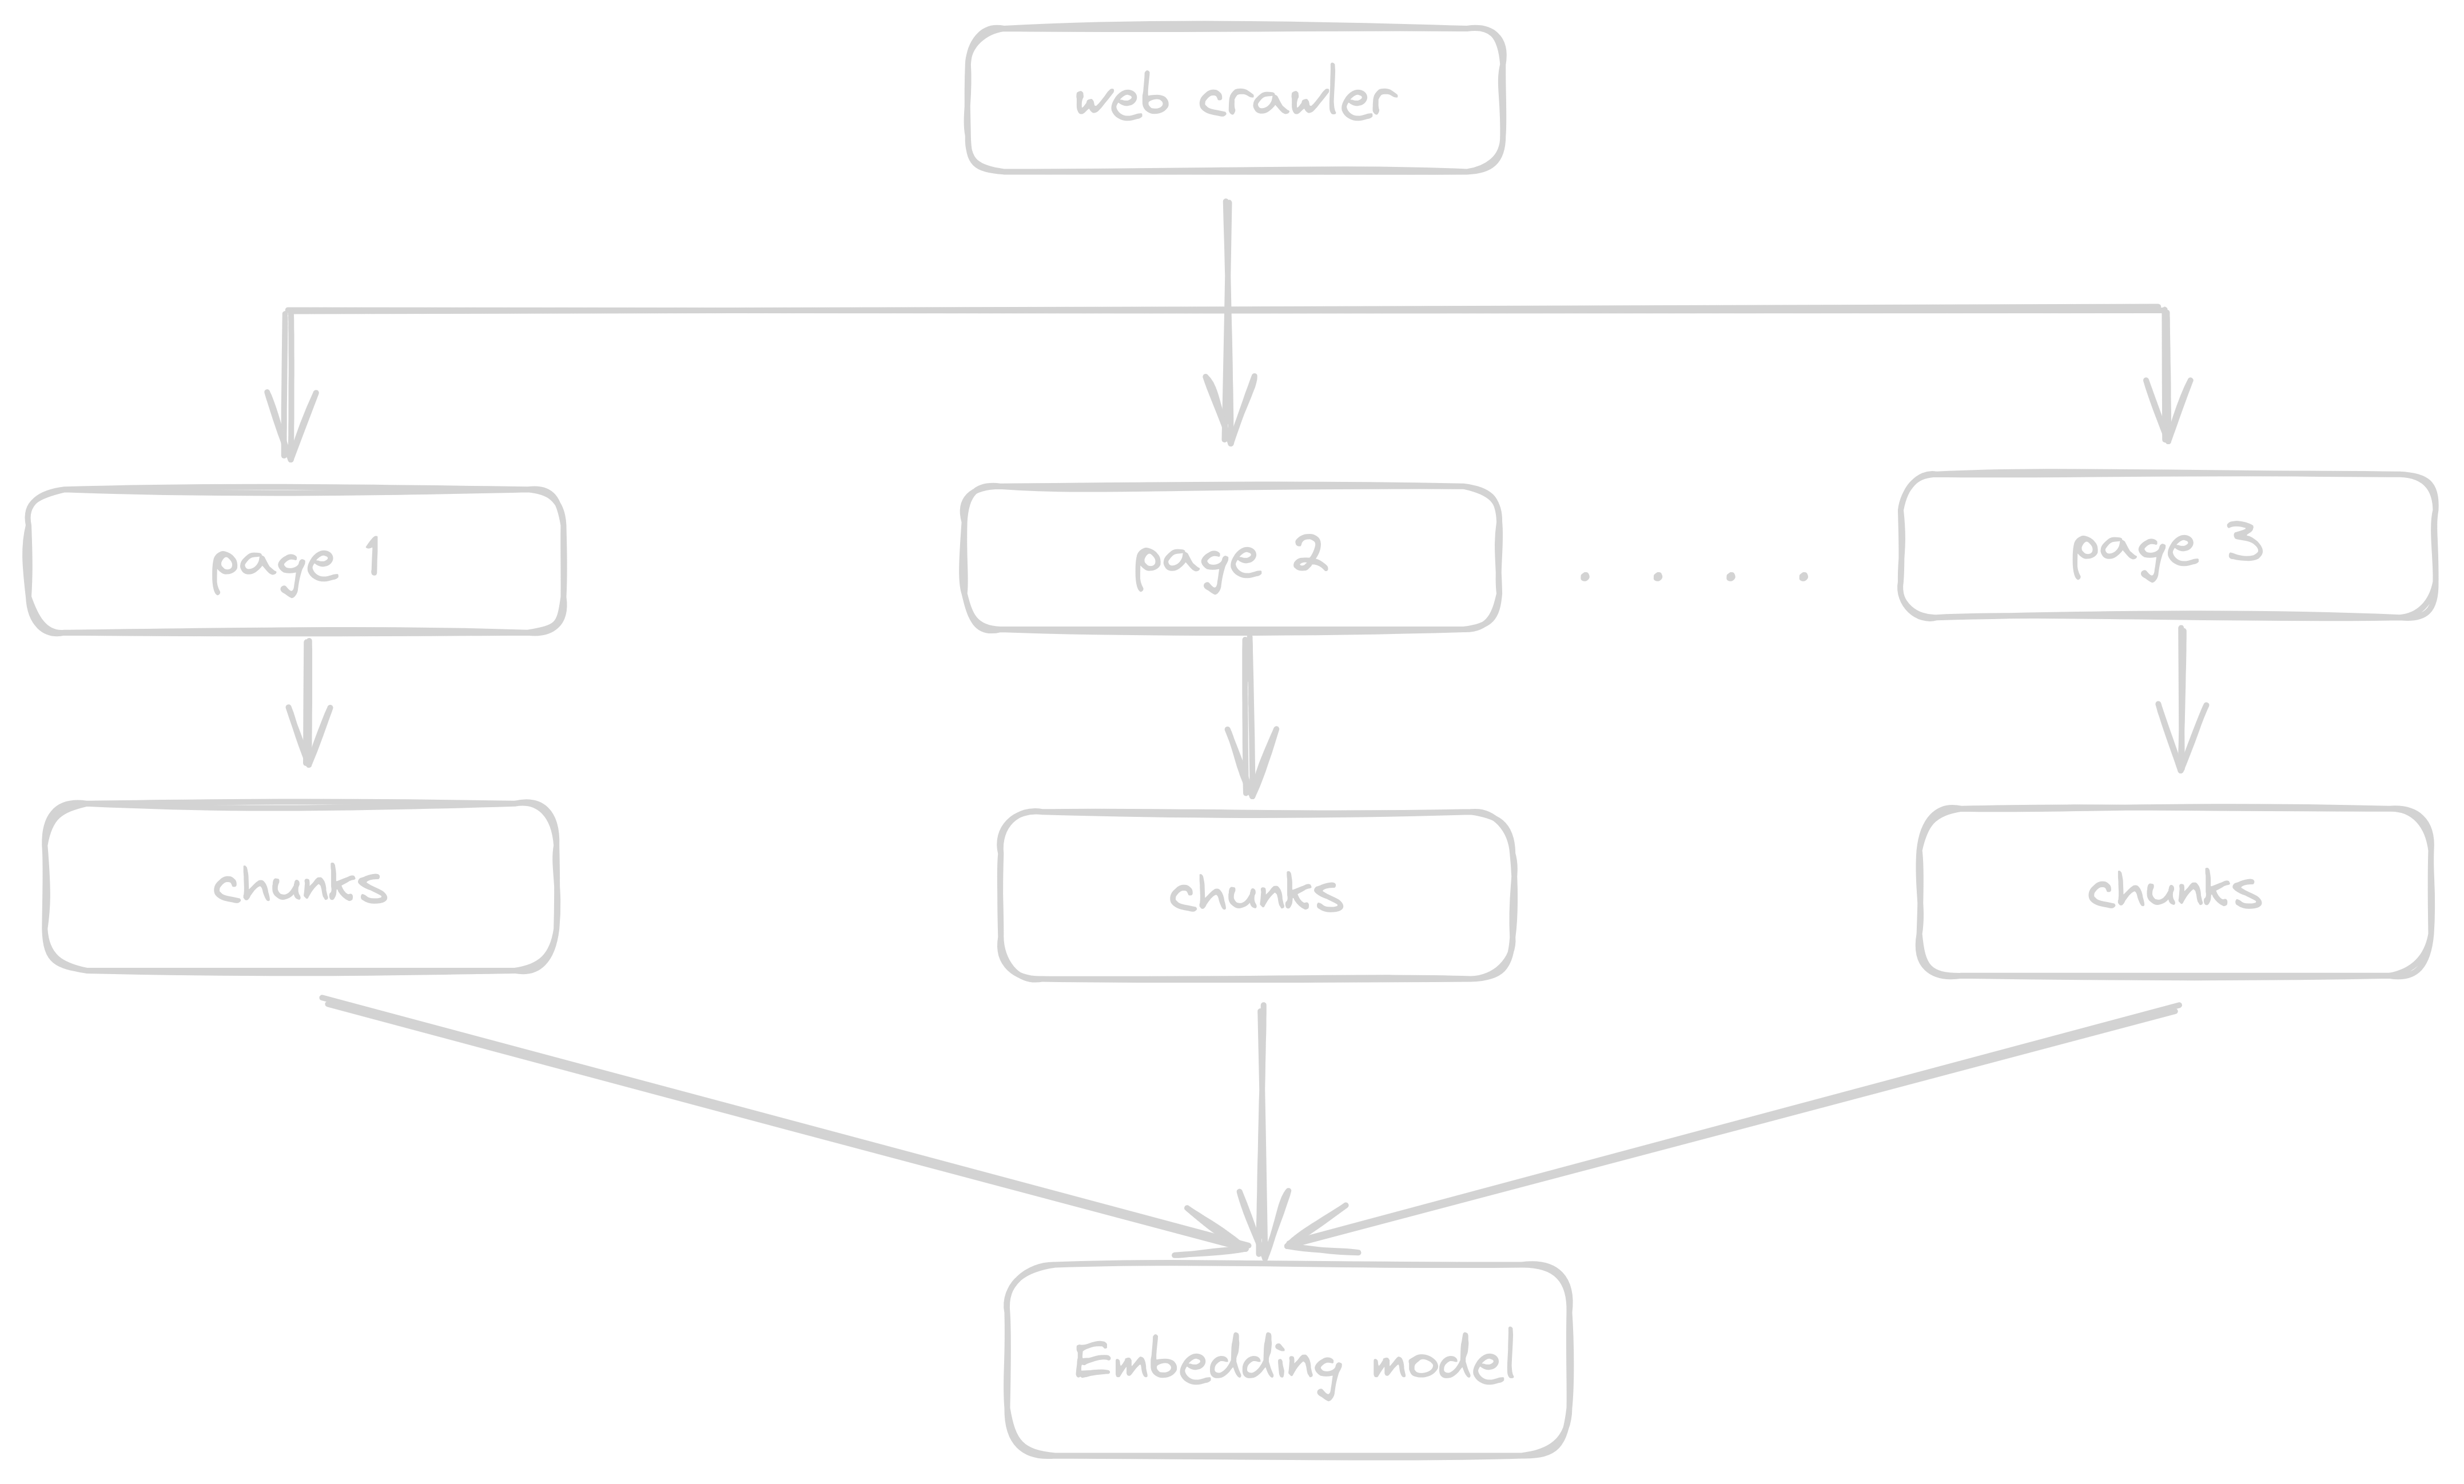
\includegraphics[width=0.8\textwidth]{crawler.png}\caption[]{Crawling process}}
        \end{figure}
    \end{frame}

    \subsection{Retrieving stored information}
    % \begin{frame}{Retrieving stored information}
    %     Overview of how RAG is going to work in this case:
    %     \begin{itemize}
    %         \item The text content of the website is chunked and preprocessed\pause
    %         \item Embeddings of the preprocessed text are then created through an embedding model\pause
    %         \item Embeddings are stored in a vectore store like Chromadb\pause
    %         \item Depending on the prompt (query), the text chunks with the highest similarity to the prompt are retrieved\pause
    %         \item This serves as the context on which the LLM answers the query\pause
    %         \item The chatbot was built with the LangChain framework
    %     \end{itemize}
    % \end{frame}
    \begin{frame}{Retrieving stored information}
        \begin{figure}
            \centering
            \only<1>{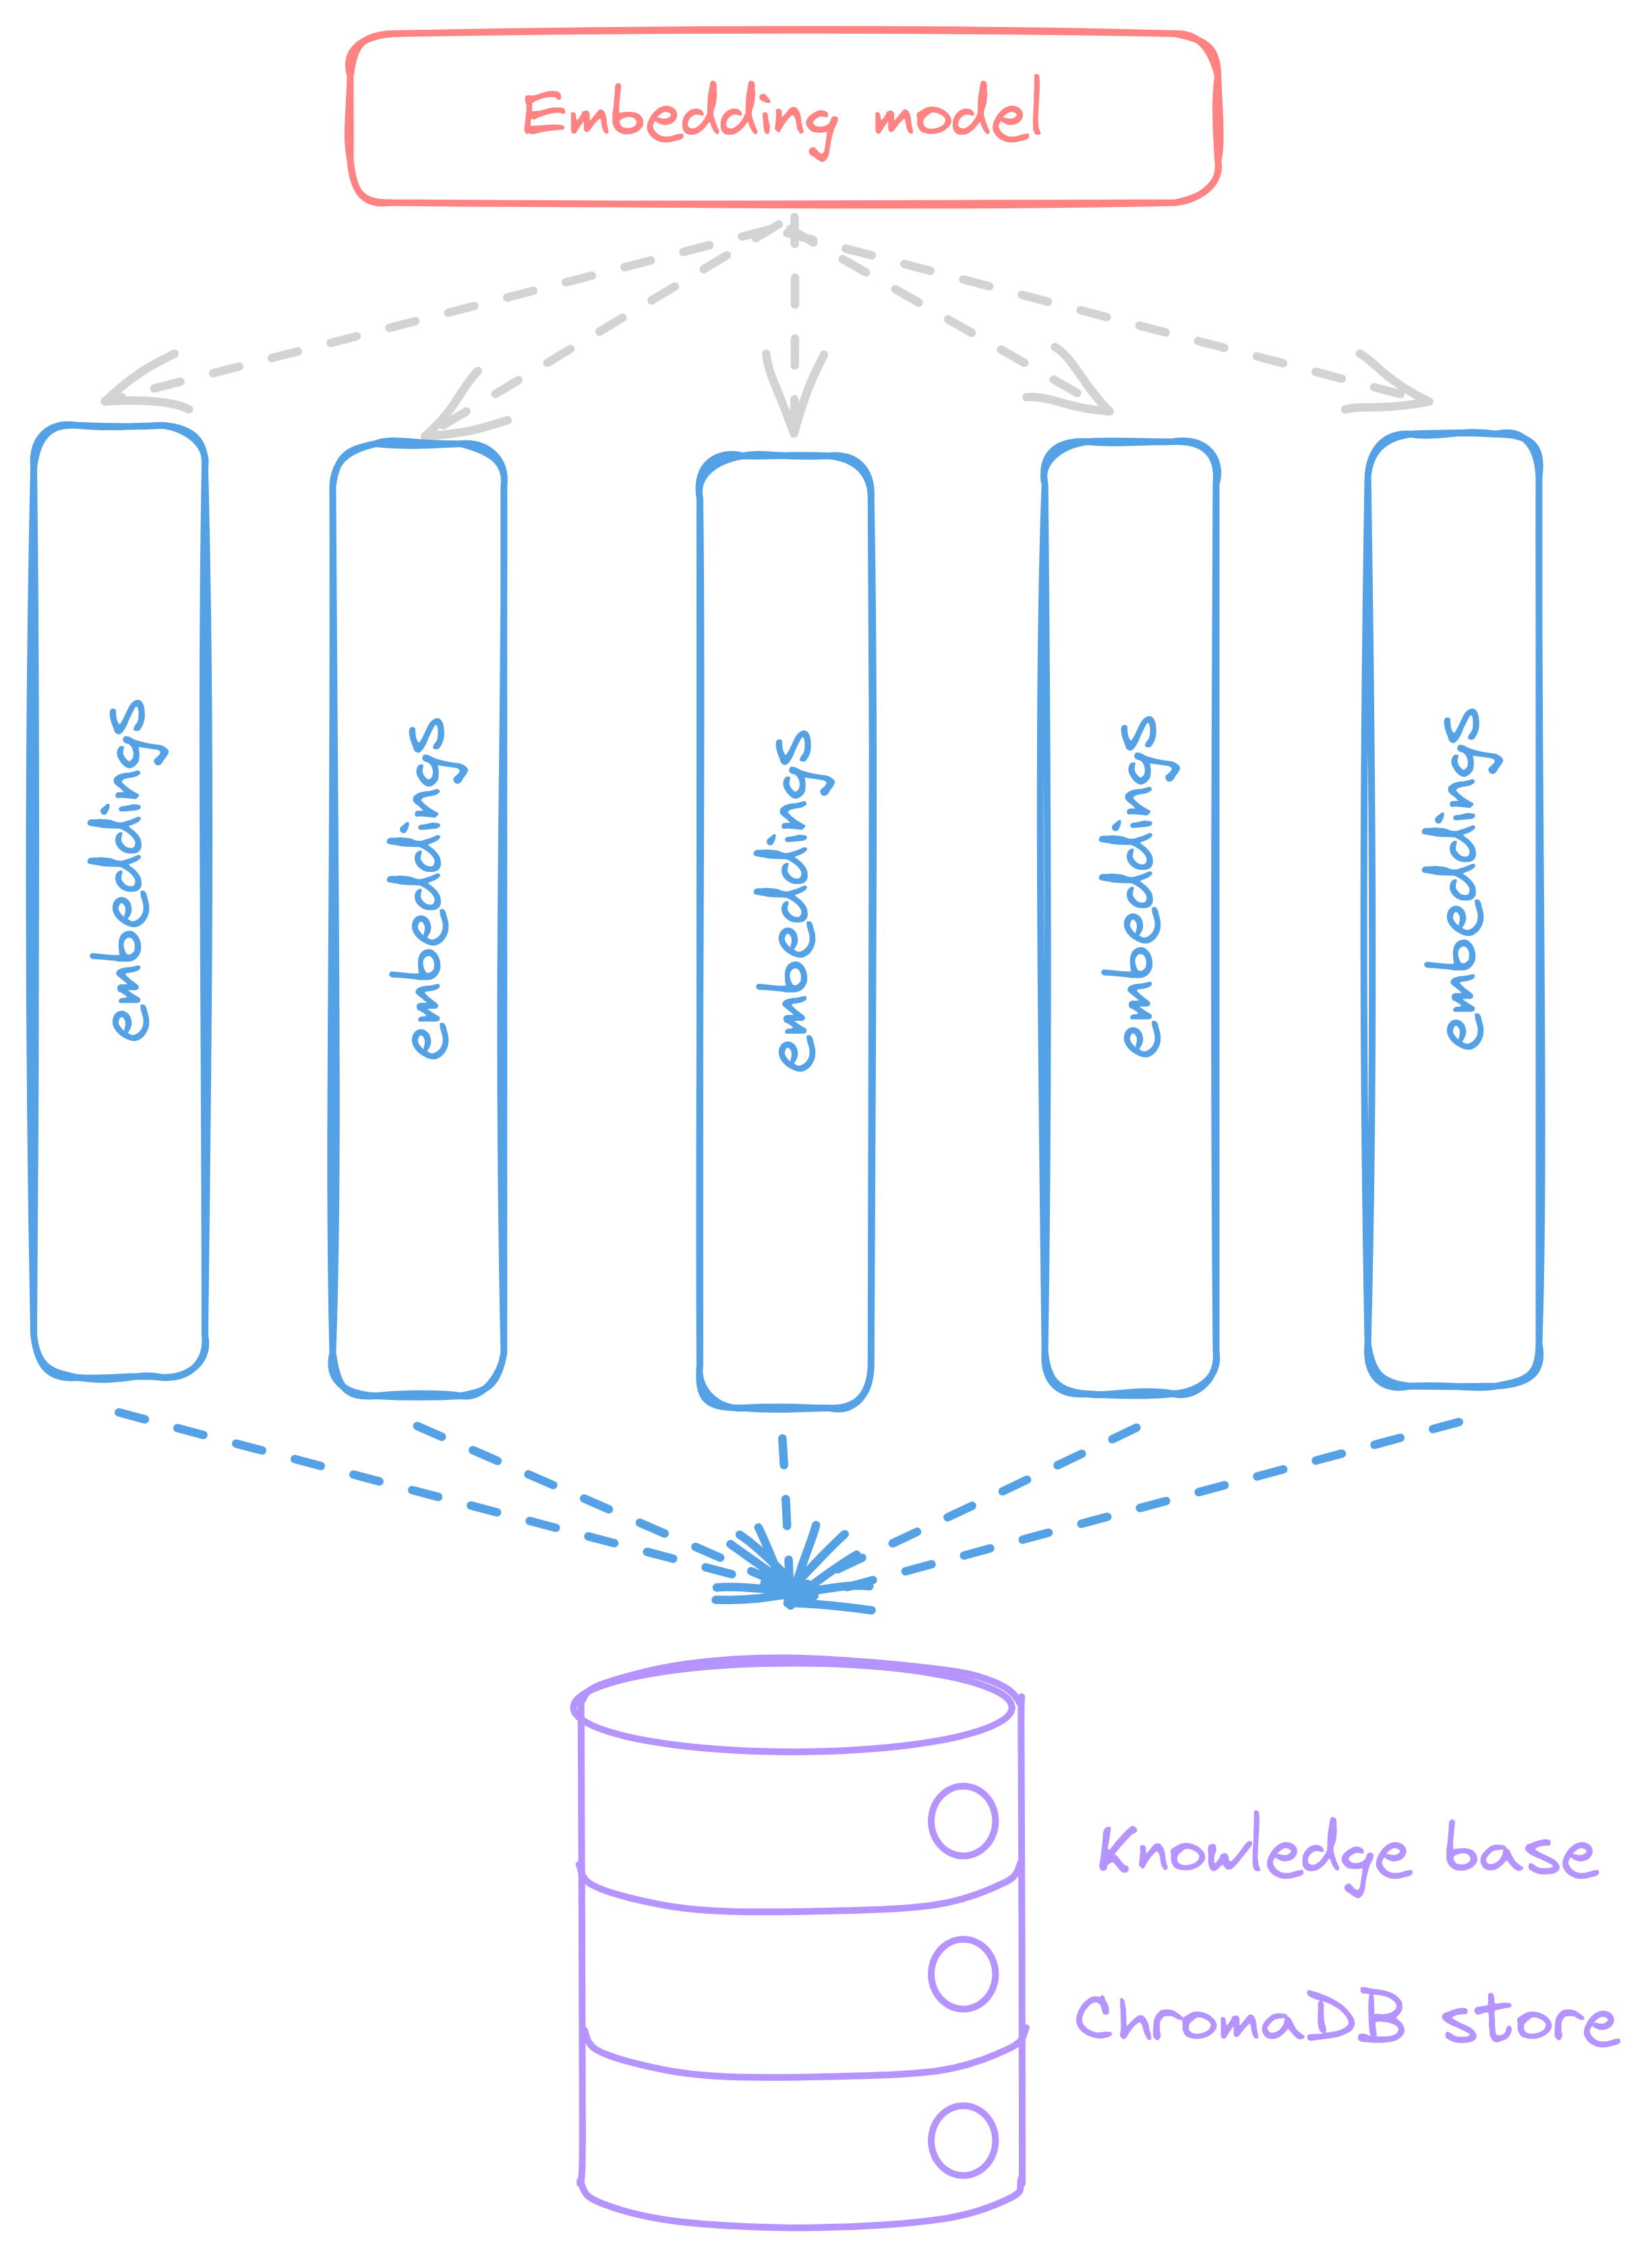
\includegraphics[height=0.8\textheight]{rag.png}}
            \only<2>{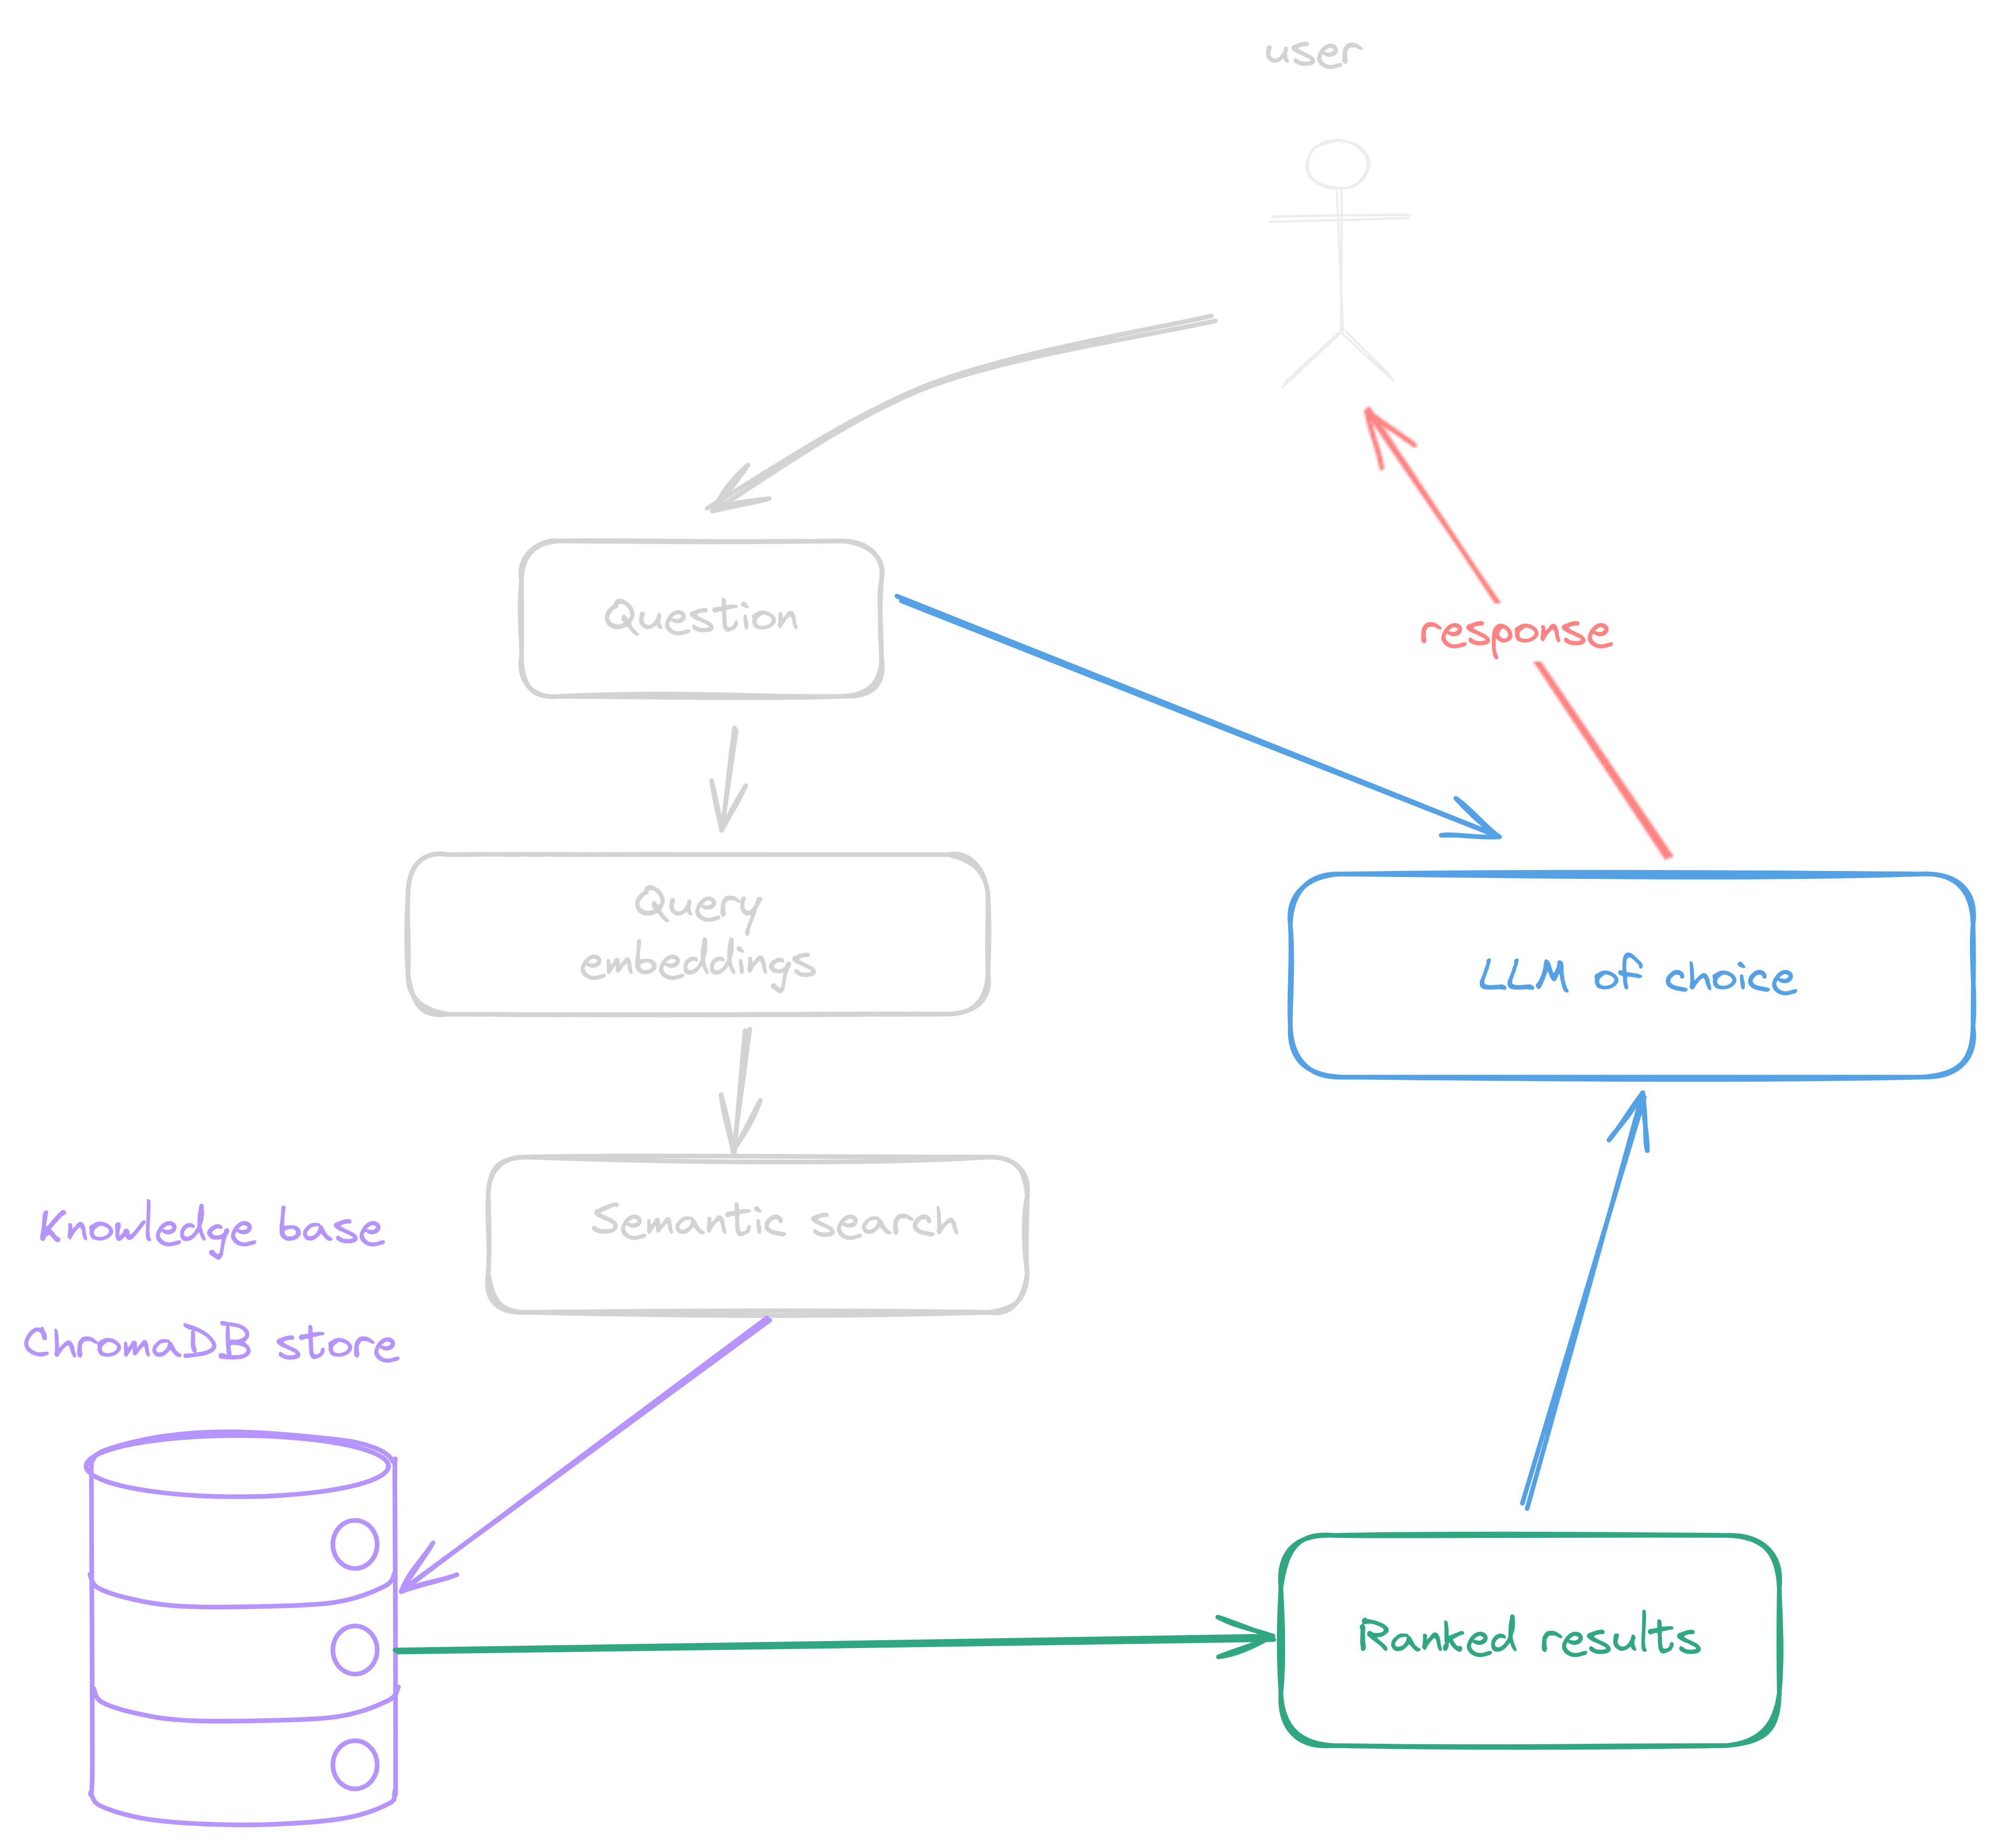
\includegraphics[height=0.8\textheight]{rag-2.png}}
        \end{figure}
    \end{frame}

    \subsection{LLM's used}
    \begin{frame}{LLM's used}
        \begin{itemize}
            \item In this work we use and compare LLM's of 3 different sizes:
            \begin{itemize}
                \item \texttt{TinyLlama 1B}
                \item \texttt{Zephyr 3B}
                \item \texttt{WizardLM 7B}
            \end{itemize}
            \item Each of the models are downloaded and loaded in 8-bit precision after quantization. This is done to reduce GPU memory footprint.
            \item We use \texttt{e5-large-v2} sentence embeddings. The embedding dimension is 1024.
            \item Finally we compare the outputs of the 3 LLM's on the same prompt.
            \item The pipeline was built with the LangChain framework.
        \end{itemize}
    \end{frame}

    \section{Comparison of results}
    \begin{frame}{Comparison of results}
        \textbf{Prompt}: \textit{Give the cooking procedure (with ingredients and instructions) for a chicken curry dish in the cookbook.}
        \begin{figure}
            \only<1>{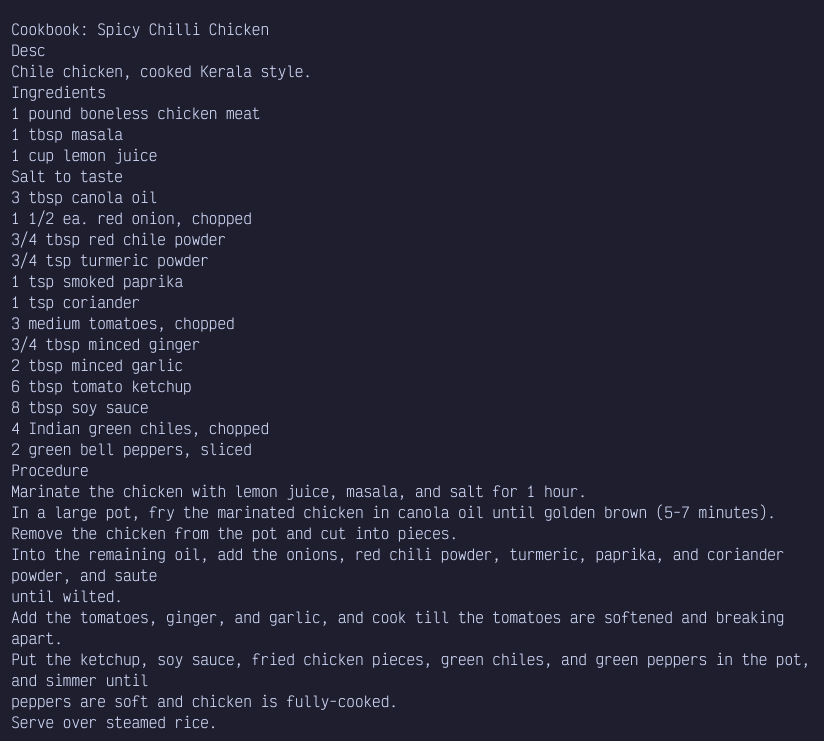
\includegraphics[height=0.6\textheight]{q1-1b.png}\caption[]{TinyLlama 1B}}
            \only<2>{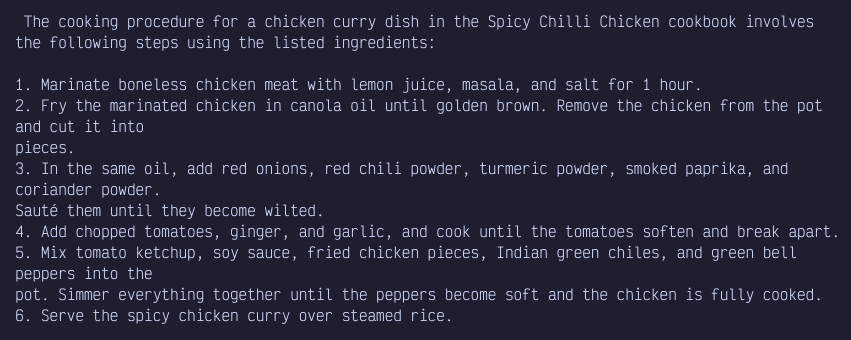
\includegraphics[width = 0.8\textwidth]{q1-3b.png}\caption[]{Zephyr 3B}}
            \only<3>{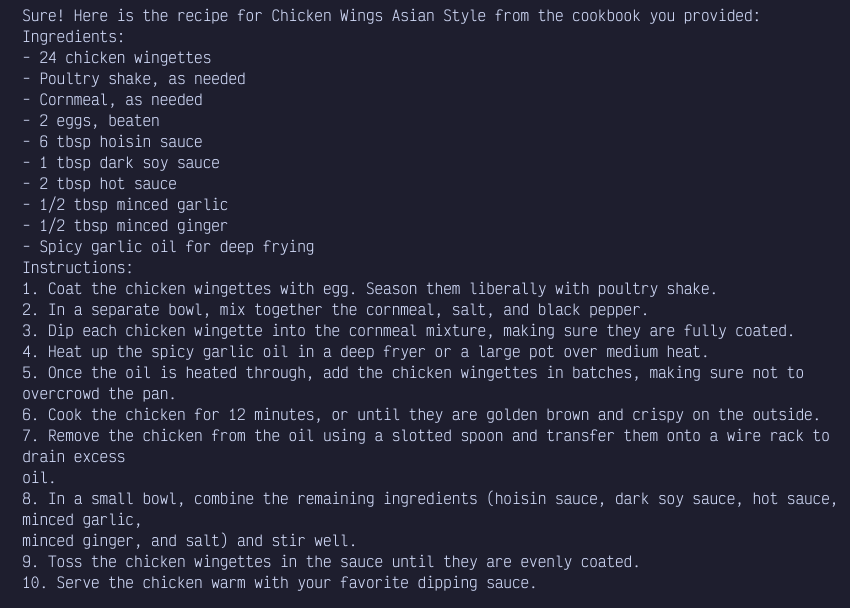
\includegraphics[height=0.6\textheight]{q1-7b.png}\caption[]{WizardLM 7B}}
        \end{figure}
    \end{frame}

    \begin{frame}{Comparison of results}
        \textbf{Prompt}: \textit{Give the ingredients for an Asian spicy dish in the cookbook}
        \begin{figure}
            \only<1>{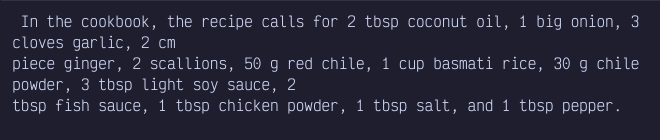
\includegraphics[width=0.8\textwidth]{q2-1b.png}\caption[]{TinyLlama 1B}}
            \only<2>{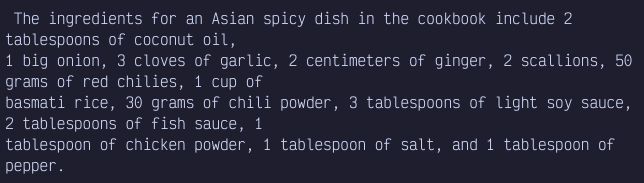
\includegraphics[width = 0.8\textwidth]{q2-3b.png}\caption[]{Zephyr 3B}}
            \only<3>{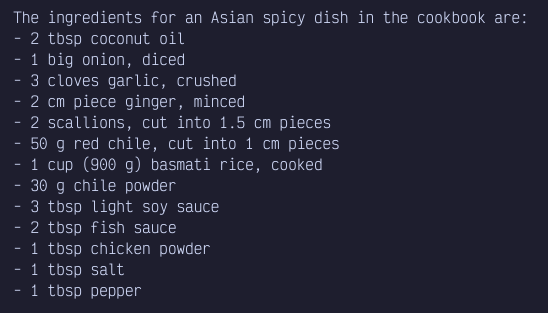
\includegraphics[height=0.6\textheight]{q2-7b.png}\caption[]{WizardLM 7B}}
        \end{figure}
    \end{frame}

    % \begin{frame}{Comparison of results}
    %     \textbf{Prompt}: \textit{Give the cooking procedure (with ingredients and instructions) for a chicken curry dish in the cookbook.}
    %     \begin{figure}
    %         \only<1>{\includegraphics[height=0.5\textwidth]{q3-1b.png}\caption[]{TinyLlama 1B}}
    %         \only<2>{\includegraphics[width = 0.6\textwidth]{q3-3b.png}\caption[]{Zephyr 3B}}
    %         \only<3>{\includegraphics[height=0.5\textwidth]{q3-7b.png}\caption[]{WizardLM 7B}}
    %     \end{figure}
    % \end{frame}

    \begin{frame}{Comparison of results}
        \begin{itemize}
            \item We see that the 7B model gives much more verbose and well-formatted results than the smaller models.
            \item However in the scale of sizes of LLM's, size difference between 1B, 3B, 7B is not so significant.
            \item Hence we do not see extremely large differences between their performances
            \item However in some cases, the smaller models execute faster than the bigger models.
            \item In some of the inferences regarding listing some recipes, the smaller models tend to hallucinate, but the larger models do not.
        \end{itemize}
    \end{frame}

    \section{Conclusion}
    \subsection{Challenges and trade-offs}
    \begin{frame}{Challenges and trade-offs}
        We faced the following challenges:
        \begin{itemize}
            \item LLM models are prone to hallucinate, even when feeding a context with RAG
            \item The process is GPU intensive, and required us to use platforms such as colab and kaggle
            \item There is a trade-off of performance vs cost - OpenAI api's are better but expensive than the free alternatives
            \item There is a trade-off of performance vs compute - because of less availibility of GPU memory, we can only experiment with smaller models
        \end{itemize}
    \end{frame}

    \subsection{Division of responsibilities}
    \begin{frame}{Division of responsibilities}
        \begin{table}
            \centering
            \begin{tabular}{|l|p{20em}|}
                \hline
                \textbf{Name}   &   \textbf{Responsibility} \\\hline
                Ujan Dasgupta   &   Web scraping, data preprocessing and preparation\\\hline
                Subhashree Saha &   Building the pipeline and chatbot framework with Langchain\\\hline
                Soham Sengupta  &   Experiment performance of different LLM's on different queries\\\hline
                Roudranil Das   &   Web scraping, code versioning and making the PPT\\\hline
                
            \end{tabular}
        \end{table}
    \end{frame}

    \begin{frame}
        \vfill
        \centering
        {\Large Code Walkthrough}
        \vfill
    \end{frame}

\end{document}